\begin{center}
 {\it{by Amin Aboubrahim and 
Pran Nath
}}
\end{center}




In this section, we discuss the potential of HL-LHC and HE-LHC for discovering a heavy charged Higgs boson~\cite{Aboubrahim:2018tpf} ($m_{H^{\pm}} > m_t$) in a class of high scale models, specifically SUGRA models~\cite{Chamseddine:1982jx,Nath:1983aw,Hall:1983iz} (for a review see~\cite{Nath:2016qzm}) consistent with the experimental constraints on the light Higgs mass at $\sim 125$ \UGeV and dark matter relic density (for a recent related work see~\cite{Aboubrahim:2018bil}).  We will focus on models where the
radiative  electroweak symmetry breaking is likely realised on the hyperbolic branch~\cite{Chan:1997bi}
and where the Higgs mixing parameter $\mu$ can be relatively small. Specifically we consider supergravity models with  non-universalities in  the Higgs sector and in the gaugino sector so that 
the extended parameter space of the models we consider is given by $m_0, ~A_0, ~m_1, ~m_2, ~m_3, ~m^0_{H_u}, ~m^0_{H_d}, ~\tan\beta, ~\text{sgn}(\mu)$.
Here $m_0$ is the universal scalar mass, $A_0$ is the universal trilinear coupling, 
$m_1,  m_2, m_3$ are the masses of the $U(1)$, $SU(2)$, and $SU(3)_C$ gauginos, and $m^0_{H_u}$ and $m^0_{H_d}$ are the 
masses of the up and down Higgs bosons all at the GUT scale. To satisfy the relic density constraint in these models often
one needs  co-annihilation (see, e.g.,~\cite{Aboubrahim:2017aen,Aboubrahim:2017wjl} and the references therein).

The largest production mode of the charged Higgs at hadron colliders is the one that proceeds in association with a top quark (and a low transverse momentum $b$-quark), $pp \rightarrow t[b]H^{\pm}+X$. This production mode can be realised in two schemes, namely, the four and five flavour schemes (4FS and 5FS, respectively), where in the former, the $b$-quark is produced in the final state and  in the latter it is considered as part of the proton's sea of quarks and folded into the parton distribution functions. The cross-sections of the two production modes $q\bar{q}, gg \rightarrow tbH^{\pm} ~\text{(4FS)}$ and $gb \rightarrow tH^{\pm} ~\text{(5FS)}$, are evaluated at next-to-leading order (NLO) in QCD with \code{MadGraph\_aMC@NLO-2.6.3}~\cite{Alwall:2014hca} using \code{FeynRules}~\cite{Alloul:2013bka} UFO files~\cite{Degrande:2011ua,Degrande:2014vpa} for the Type-II 2HDM. The simulation is done at fixed order, i.e., no matching with parton shower. The couplings of the 2HDM are the same as in the MSSM, but when calculating production cross-sections in the MSSM, one should take into account the SUSY-QCD effects. In our case, gluinos and stops are rather heavy and thus their loop contributions to the cross-section are very minimal. In this case, the 2HDM is the decoupling limit of the MSSM and this justifies using the 2HDM code to calculate cross-sections. For the 5FS, the bottom Yukawa coupling is assumed to be non-zero and normalised to the on-shell running $b$-quark mass. In the 5FS, the process is initiated via gluon-$b$-quark fusion while in the 4FS it proceeds through either quark-antiquark annihilation (small contribution) or gluon-gluon fusion. At finite order in perturbation theory, the cross-sections of the two schemes do not match due to the way the perturbative expansion is handled but one expects to get the same results for 4FS and 5FS when taking into account all orders in the perturbation. In order to combine both estimates of the cross-section, we use the Santander matching criterion~\cite{Harlander:2011aa} whereby 
\begin{equation}
\sigma^{\rm matched}= ({\sigma^{4\rm FS}+\alpha\sigma^{5\rm FS}})/{1+\alpha},
\label{matched}
\end{equation}  
with $\alpha=\ln\left(\frac{m_{H^{\pm}}}{\bar{m}_b}\right)-2$. The uncertainties are combined as $\delta\sigma^{\rm matched}=\frac{\delta\sigma^{4\rm FS}+\alpha\delta\sigma^{5\rm FS}}{1+\alpha}$. The results are shown in Table~\ref{tab1:xsec}.


\begin{table}[th]
\begin{center}
\resizebox{\linewidth}{!}{\begin{tabulary}{1.12\textwidth}{l|CC|CC|CC|CC}
\hline\hline\rule{0pt}{3ex}
Model  & \multicolumn{2}{c}{$\sigma^{\rm 4FS}_{\rm NLO}(pp\rightarrow tbH^{\pm})$} & \multicolumn{2}{c}{$\sigma^{\rm 5FS}_{\rm NLO}(pp\rightarrow tH^{\pm})$} & \multicolumn{2}{c}{$\sigma^{\rm matched}_{\rm NLO}$} & $\mu_F=\mu_R$ & $\bar{m}_b$\\
  & 14 \UTeV & 27 \UTeV & 14 \UTeV & 27 \UTeV  & 14 \UTeV & 27 \UTeV & \multicolumn{2}{c}{(\UGeV)} \\ 
\hline\rule{0pt}{3ex} 
\!\!(a) & 49.0$^{+12.6\%}_{-13.1\%}$ & 272.8$^{+9.2\%}_{-10.3\%}$ & 71.8$^{+6.6\%}_{-5.7\%}$ & 397.1$^{+7.0\%}_{-6.6\%}$  & 65.9$^{+8.1\%}_{-7.6\%}$ & 365.4$^{+7.6\%}_{-7.5\%}$ & 183.6 & 2.72  \\
(b)  & 34.5$^{+10.6\%}_{-12.1\%}$ & 204.6$^{+8.1\%}_{-9.6\%}$ & 58.3$^{+7.0\%}_{-5.9\%}$ & 336.1$^{+6.9\%}_{-6.5\%}$ & 52.4$^{+7.9\%}_{-7.4\%}$ & 303.5$^{+7.2\%}_{-7.3\%}$ & 197.9 & 2.70  \\
(c)  & 29.1$^{+11.1\%}_{-12.3\%}$ & 175.9$^{+8.2\%}_{-9.7\%}$ & 48.8$^{+6.7\%}_{-5.7\%}$ & 285.9$^{+6.4\%}_{-6.0\%}$ & 43.9$^{+7.8\%}_{-7.3\%}$ & 259.0$^{+6.8\%}_{-6.9\%}$ & 205.6 & 2.69 \\
(d) & 24.8$^{+10.9\%}_{-12.3\%}$ & 149.9$^{+7.1\%}_{-9.1\%}$ & 42.6$^{+6.3\%}_{-5.3\%}$ & 264.8$^{+6.8\%}_{-6.2\%}$ & 38.3$^{+7.4\%}_{-6.9\%}$ & 237.2$^{+6.8\%}_{-6.9\%}$ & 215.9 & 2.68 \\
(e) & 18.4$^{+11.2\%}_{-12.4\%}$ & 120.1$^{+8.3\%}_{-9.8\%}$ & 32.3$^{+5.9\%}_{-4.9\%}$ & 206.7$^{+6.4\%}_{-6.0\%}$ & 29.0$^{+7.1\%}_{-6.7\%}$ & 186.3$^{+6.8\%}_{-6.9\%}$ & 229.6 & 2.67 \\
(f)  & 13.6$^{+11.3\%}_{-12.5\%}$ & 93.2$^{+7.8\%}_{-9.5\%}$ & 25.1$^{+6.1\%}_{-5.2\%}$ & 169.6$^{+6.7\%}_{-6.0\%}$ & 22.4$^{+7.3\%}_{-6.9\%}$ & 152.1$^{+7.0\%}_{-6.8\%}$ & 248.2 & 2.65  \\
(g) & 13.1$^{+10.5\%}_{-12\%}$ & 95.8$^{+7.6\%}_{-9.5\%}$ & 26.0$^{+6.2\%}_{-5.6\%}$ & 185.1$^{+6.7\%}_{-6.0\%}$ & 23.1$^{+7.2\%}_{-7.0\%}$ & 165.0$^{+6.8\%}_{-6.8\%}$ & 264.6 & 2.64 \\
(h) & 11.2$^{+10.3\%}_{-12.0\%}$ & 85.1$^{+7.5\%}_{-9.4\%}$ & 22.7$^{+6.1\%}_{-5.8\%}$ & 168.3$^{+6.8\%}_{-5.9\%}$ & 20.2$^{+7.0\%}_{-7.2\%}$ & 149.9$^{+6.9\%}_{-6.7\%}$ & 278.2 & 2.63 \\
(i)  & 7.8$^{+11.7\%}_{-12.6\%}$ & 61.1$^{+8.1\%}_{-9.8\%}$ & 15.8$^{+6.0\%}_{-6.0\%}$ & 121.0$^{+6.9\%}_{-6.0\%}$ & 14.0$^{+7.2\%}_{-7.4\%}$ & 107.9$^{+7.2\%}_{-6.8\%}$ & 292.9 & 2.62 \\
(j) & 5.5$^{+12.6\%}_{-13.0\%}$ & 48.9$^{+9.1\%}_{-10.3\%}$ & 11.6$^{+6.7\%}_{-6.5\%}$ & 99.4$^{+6.4\%}_{-5.5\%}$ & 10.3$^{+7.9\%}_{-7.8\%}$ & 88.7$^{+6.9\%}_{-6.5\%}$ & 329.9 & 2.60 \\
\hline
\end{tabulary}}\end{center}
\caption{The NLO production cross-sections, in fb, of the charged Higgs in association with a top (and bottom) quark in the five (and four) flavour schemes along with the matched values at $\sqrt{s}=14$ \UTeV and $\sqrt{s}=27$ \UTeV for the ten benchmark points in~\cite{Aboubrahim:2018tpf}. The running $b$-quark mass, $\bar{m}_b$, is also shown evaluated at the factorisation and normalisation scales, $\mu_F=\mu_R=\frac{1}{3}(m_t+\bar{m}_b+m_{H^{\pm}})$.}
\label{tab1:xsec}
\end{table}

For the parameter points considered, the $H^{\pm}\rightarrow\tau\nu$ channel has the smallest branching ratio but it is of interest since jets can be tau-tagged and the tau has leptonic and hadronic decay signatures. For the considered signal final states (fully hadronic), the SM backgrounds are mainly $t\bar{t}$, $t$+jets, $W/Z/\gamma^*$+jets, di-boson production and QCD multi-jet events which can fake the hadronic tau decays. The simulation of the charged Higgs associated production, $t[b]H^{\pm}$, is done at fixed order in NLO while the SM backgrounds are done at LO (which are then normalised to their NLO values) using \code{MadGraph} interfaced with LHAPDF~\cite{Buckley:2014ana} and \code{PYTHIA8}~\cite{Sjostrand:2014zea} which handles the showering and hadronisation of the samples.  For the SM backgrounds a five-flavor MLM matching~\cite{Mangano:2006rw} is performed on the samples. Detector simulation and event reconstruction is performed by \code{DELPHES-3.4.2}~\cite{deFavereau:2013fsa} using the beta card for HL-LHC and HE-LHC studies.

The selection criteria depends on the flavour scheme under consideration. For the 4FS (5FS) we apply a lepton veto and at least five (four) jets, two (one) of which are (is) b-tagged and one is tau-tagged. To discriminate the signal from background we use gradient boosted decision trees, \code{GradientBoost}, which proves to be more powerful than the conventional cut-based analysis. A large set of variables have been tried in the BDT training and the ones which produced the best results were kept. The kinematic variables entering into the training of the BDTs are: 
\begin{align}
E^{\rm miss}_T, ~~~ E^{\rm miss}_T/\sqrt{H_T}, ~~~m_{T2}^{\rm jets}, ~~~m_T^{\tau}, ~~~p_T^{\tau}, ~~~E^{\rm miss}_T/m_{\rm eff},  \nonumber \\
m_T^{\rm min}(j_{1-2},E^{\rm miss}_T), ~~~\Delta\phi(p^{\tau}_T,E^{\rm miss}_T), ~~~N_{\rm tracks}^{\tau}, ~~~\sum_{\rm tracks} p_T \, .
\end{align}
The training and testing of the samples is carried out using \code{ROOT}'s~\cite{Antcheva:2011zz} own TMVA (Toolkit for Multivariate Analysis) framework~\cite{Speckmayer:2010zz}. After the training and testing phase, the variable ``BDT score" is created. We apply the selection criteria (as given in~\cite{Aboubrahim:2018tpf}) along with a BDT score cut $>0.95$ on the SM background and on each of the 4FS and 5FS signal samples to obtain the remaining cross-sections. The signal cross-sections are combined using Eq.~(\ref{matched}) in order to evaluate the required minimum integrated luminosity for a $\frac{S}{\sqrt{S+B}}$ discovery at the $5\sigma$ level. The results for both the 14 and 27 \UTeV cases are shown in Fig.~\ref{fig1}. 

\begin{figure}[H]
 \centering
   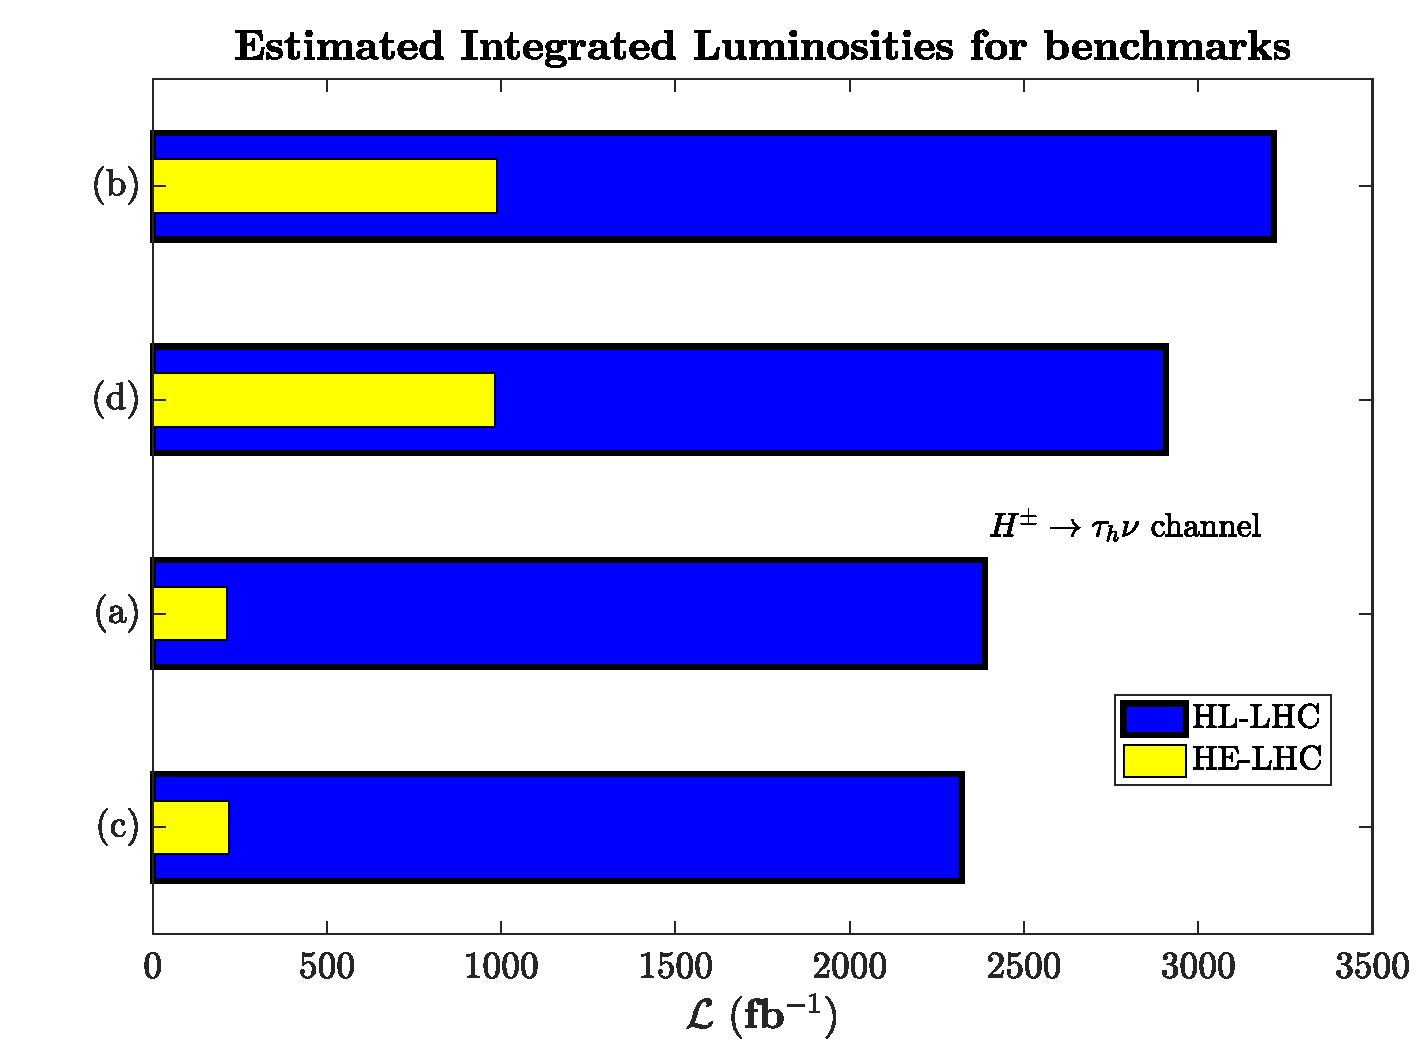
\includegraphics[width=0.49\textwidth]{\main/section9/plots/lumi_1.pdf} 
      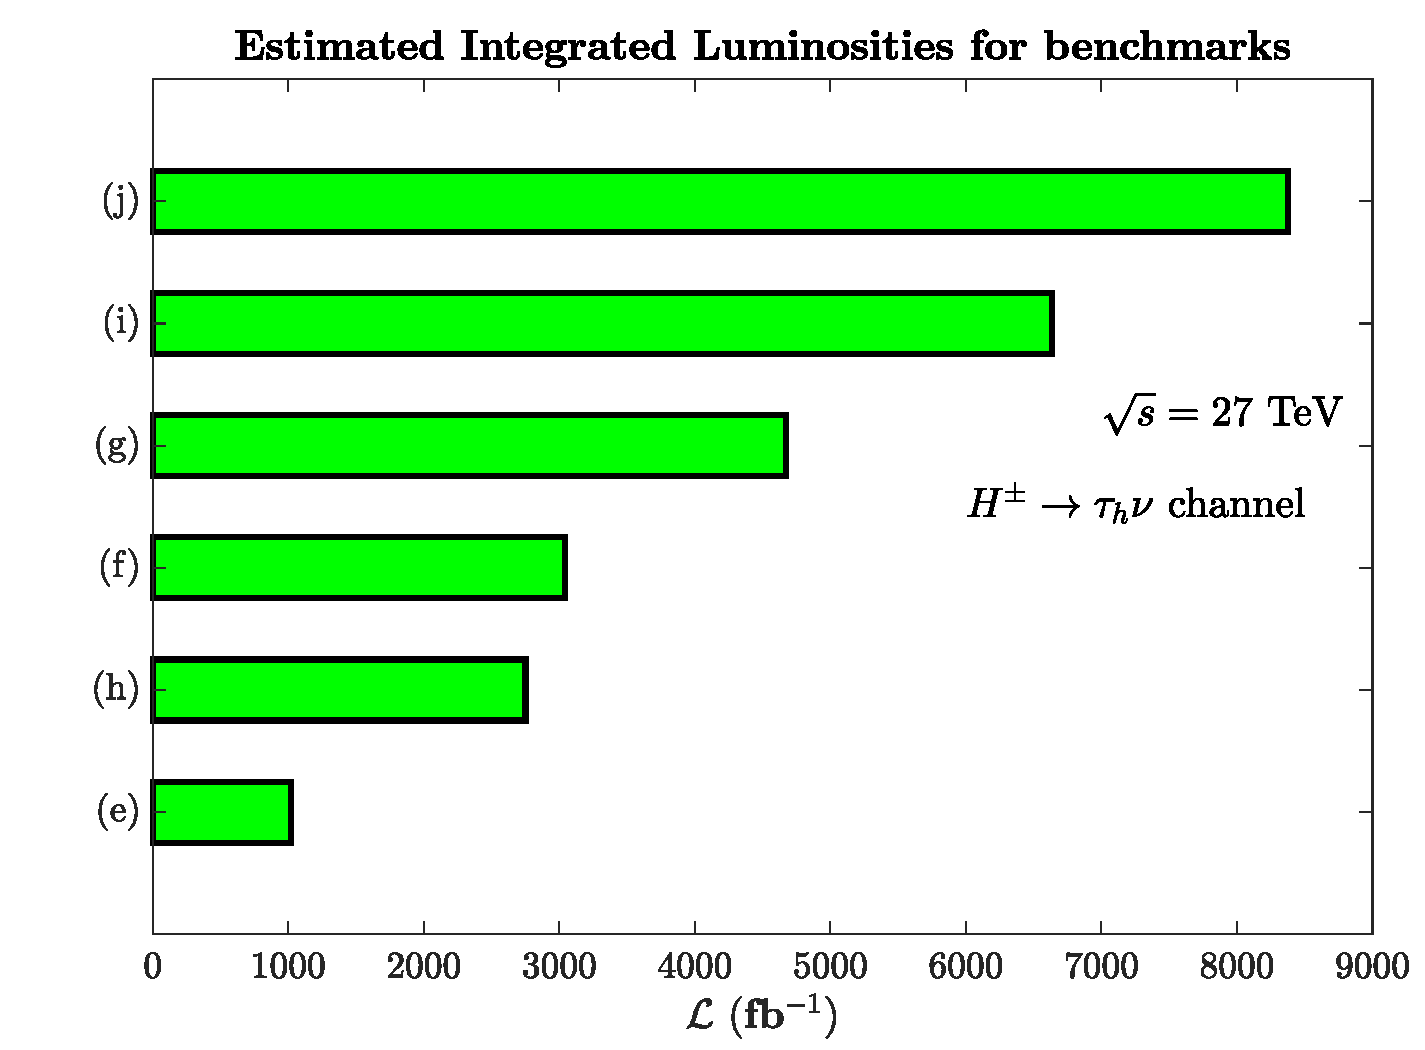
\includegraphics[width=0.49\textwidth]{\main/section9/plots/lumi_2.pdf}
   \caption{The evaluated integrated luminosities, $\mathcal{L}$ ($\ifb$), for ten benchmark points. Left plot: calculated $\mathcal{L}$ for points discoverable at both HL-LHC and HE-LHC. Right plot: calculated $\mathcal{L}$ for points discoverable only at HE-LHC.}
	\label{fig1}
\end{figure}

One can see from Fig.~\ref{fig1} that four of the ten points may be discoverable at the HL-LHC as it nears the end of its run where a maximum integrated luminosity of 3000$\ifb$ will be collected. Given the rate at which the HL-LHC will be collecting data, points (a)-(d) will require $\sim 7$ years of running time. On the other hand, the results from the 27 \UTeV collider show that all points may be discoverable for integrated luminosities much less than $15\iab$. %The HE-LHC will be collecting data at a rate of $\sim 820\ifb$ per year and with that points (a) and (c) may be discoverable within the first 3 months of operation, points (b), (d) and (e) may take $\sim 1.2$ years, points (h) and (f) $\sim 3.5$ years and the rest of the points $>6$ years.  


\textbf{Acknowledgements:}
This research was supported in part by the NSF Grant PHY-1620575.
